\documentclass[dvipdfmx, 12pt]{beamer}
\usepackage{pxjahyper}
\usepackage{minijs}
\usepackage{otf}
\renewcommand{\kanjifamilydefault}{\gtdefault}
\usetheme{Antibes}
\setbeamertemplate{navigation symbols}{}
\usepackage{url}
\usepackage{graphicx}
\usepackage{amsmath}
\usepackage{bm}
\usepackage{ascmac}
\setbeamertemplate{footline}[frame number] 


\title{Understanding Financial Crises\\Ch10 : Contagion 後半}
\author{Kei Ikegami}

\begin{document}
\newcommand{\argmin}{\mathop{\rm arg~min}\limits}

\frame{\maketitle}

\section*{目次}
\begin{frame} \frametitle{発表の流れ}
\tableofcontents
\end{frame}

\begin{frame}\frametitle{何をするか}
	\begin{itemize}
	\item 銀行間のつながりがincomplete networkでもfirst bestを達成することはできた。しかし世界全体での流動性需要量が想定される量よりも多くなる想定外の事象の下では、incomplete networkだとbankruptが地域を超えて連鎖するContagionが発生する。ということの確認。
	\item Contagionが全地域に拡大すると世界に存在する資産の価値が低下するのでやだ!ということの確認。
	\item 銀行のデータを使ってContagionが発生する規模をシミュレーションする研究の紹介。
	\end{itemize}
\end{frame}

\begin{frame}\frametitle{Pecking Order}
	\begin{itemize}
	\item date1において流動性需要が発生したときに、当該地域の銀行はどのようにして対処するかを考える。
	\item 銀行の持ってる資産は、short asset ($y$), 他銀行へのdeposits ($z$), long asset ($x$)の三種類。
	\item この三つをそれぞれ流動化して流動性を供給するわけだが、この三つは無差別ではない。
	\end{itemize}
\end{frame}

\begin{frame}\frametitle{Pecking Order : Cost of short asset}
	\begin{itemize}
	\item short assetを流動化する際のコストを考える。
	\item date 1で1の消費をもたらすshort assetの量は1である。
	\item このdate1で1の消費をもたらすだけのshort assetを使ってdate2で消費しようとすれば、買い替えによってdat2でも1だけの消費をすることができる。
	\item つまり、date1で1の消費を得るのにdate2での1を犠牲にしている。
	\item これよりshort assetを流動化するコストは1である。
	\end{itemize}
\end{frame}

\begin{frame}\frametitle{Pecking Order : Cost of depoists}
	\begin{itemize}
	\item 他国へのdepositsを流動化する際のコストを考える。
	\item interbank市場においても各国の消費者と銀行が結ぶのと同様の契約によって預金がなされているとする。
	\item すなわち、ある銀行がdate0において1単位の財を他国の銀行に預けるということは、預けた先の銀行からdate1では$c_1$、date2では$c_2$だけの引き出しを保証されているということである。
	\item ということは、date1で$c_1$だけの流動性を供給した場合、date2での$c_2$だけの消費を犠牲にしたということになる。
	\item 従ってdepositsを流動化するコストは単位あたり$\frac{c_2}{c_1}$である。
	\end{itemize}
\end{frame}

\begin{frame}\frametitle{Pecking Order : Cost of long asset}
	\begin{itemize}
	\item long assetを流動化する際のコストを考える。
	\item short assetの時と同様に考えれば良い。
	\item date1で$r$だけの消費を供給できるだけのlong assetは、date2まで持っておけば$R$だけの消費をもたらすことができるものである。
	\item 従ってlong assetを流動化するコストは単位あたり$\frac{R}{r}$である。
	\end{itemize}
\end{frame}

\begin{frame}\frametitle{Pecking Order}
	\begin{itemize}
	\item 当然先の三つをコストが安い順に流動化していく。
	\item 銀行のFOCより$1 < \frac{c_2}{c_1}$である。
	\item $r$を十分低く設定すれば$\frac{c_2}{c_1} < \frac{R}{r}$は満たされる。
	\item よって、以下では「short asset」「他銀行へのdeposits」「long asset」の順で流動化していくと仮定する。
	\item これをPecking orderと呼ぶ。
	\end{itemize}
\end{frame}

\begin{frame}\frametitle{設定1}
	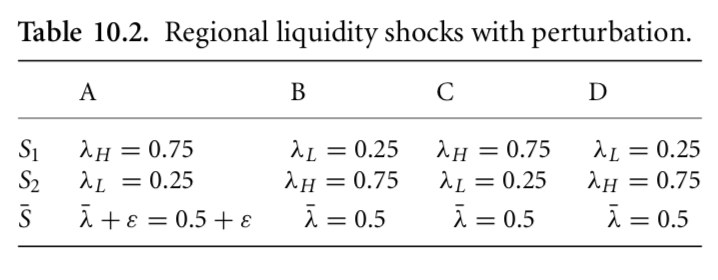
\includegraphics[width = 7cm]{10-2.png}
	
	\begin{itemize}
	\item $\bar{S}$が確率0で発生すると想定されている事象(本当はおこりうる)。
	\item $\epsilon$分だけ世界全体での流動性需要が通常の状態よりも多くなって老いることに注意。
	\item 前半同様に$(c_1, c_2) = (1, 1.5), (x,y) = (0.5, 0.5), r = 0.4$とする。
	\end{itemize}
\end{frame}

\begin{frame}\frametitle{設定2}
	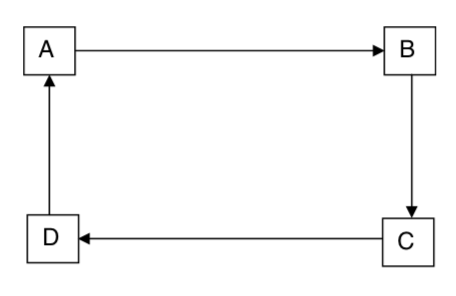
\includegraphics[width = 7cm]{10-5.png}
	\begin{itemize}
	\item interbank networkは上図のようなincomplete netwrokとなっている。
	\item 異常事態$\bar{S}$には各主体確率0を割り当てているので、$z = 0.25$だけのdepositsを矢印の向きに預けている状態である。
	\end{itemize}
\end{frame}

\begin{frame}\frametitle{想定する状況}
	\begin{itemize}
	\item 上記の設定の下で$\bar{S}$が発生した時にこの世界で何が起こるかを以下で見ていく。
	\end{itemize}
	想定するのは以下の二つの状況。
	\begin{enumerate}
	\item $\epsilon = 0.1, R = 1.5$
	\item $\epsilon = 0.1, R = 1.2$
	\end{enumerate}
	ケース1では銀行が破綻するがinterbank networkのバッファが働き、金融危機は限定された地域に止まる。しかしケース2では銀行の破綻が連鎖的に発生し、資産価値が世界的に低下する金融危機が発生する。
\end{frame}

\begin{frame}\frametitle{ケース1 : 銀行Aの動き}
	\begin{itemize}
	\item A地域におけるearly consumerの割合は0.6
	\item 銀行Aはshort assetを0.5しか持ってないので、pecking orderに従い、0.1だけB銀行のdepositsを流動化することを考える。
	\item しかし$\bar{S}$ではdate1において地域Bでも0.5だけの消費需要が発生している。
	\item 銀行Bが持つshort assetも0.5なので、銀行Aからの流動性需要に対応するためにはpecking orderに従い銀行Cのdepositsを流動化しようとする。
	\item この状況は銀行B, C, Dにおいて共通であり、巡り巡ってDからAへの流動性需要が発生する。
	\item Bから引き出しても同額をDに引き渡さないといけないのでdepositsを流動化することでは自国の流動性需要には答えられないことがわかる。
	\end{itemize}
\end{frame}

\begin{frame}\frametitle{ケース1 : 銀行Aの動き}
	\begin{itemize}
	\item Pecking orderに従い、銀行Aは次にlong assetを流動化しようとする。
	\item $0.1/0.4 = 0.25$だけlongを流動化すれば流動性需要に対処できる。
	\item これよりdate2に残ってるlongは$0.25$であり、これから$0.25 * 1.5 = 0.375$だけの財を得られる。
	\item 地域Aにおけるlate consumerは0.4だったので、一人ずつこれを割り振ると、$c_2 = 0.375 / 0.4 = 0.94$となる。
	\item date1における消費$c_1 = 1$よりもこれが少ないので、late consumerはearly consumerのふりをするインセンティブを持つ。
	\item すなわち銀行Aでは取り付け騒ぎが発生し、bank runとなる。
	\end{itemize}
\end{frame}

\begin{frame}\frametitle{ケース1 : 銀行Dの動き}
	\begin{itemize}
	\item この取り付けには銀行Aにdepositsを持つ銀行Dも巻き込まれる。
	\item しかし、このケースにおいて銀行Dもbank runとなるようなContagionは発生しない。これを以下で確認する。
	\item Contagionが発生せず、地域Dでbank runが食い止められたとする。
	\item この時、当然Bはbank runしていないので、その資産価値は目減りせず、銀行Aが銀行Bに持つdepositsの価値は$0.25$のままである。
	\item 銀行Aの資産はこの他にもshort assetとlong assetの二つがある。
	\item short assetはdate1において$0.5$だけの価値をもち、long assetは流動化により$0.5 * 0.4$だけの価値を持つ。
	\end{itemize}
\end{frame}

\begin{frame}\frametitle{ケース1 : 銀行Dの動き}
	\begin{itemize}
	\item 以上より銀行Aのdate1における総資産価値は$0.5 + 0.5 * 0.4 + 0.25 = 0.95$である。
	\item ここで銀行Aではdate1に取り付け騒ぎが起きていることを思い出す。
	\item ここで銀行Aから預金を引き出そうとするのは、地域Aに住む全住民と銀行Dの二者である。
	\item 前者は合計$1$だけ引き出そうとする。
	\item 後者は$0.25$だけ引き出そうとする。
	\item 合わせて、date1で銀行Aから引き出される総額は$1.25$である。
	\end{itemize}
\end{frame}

\begin{frame}\frametitle{}
	\begin{itemize}
	\item 
	\end{itemize}
\end{frame}

\begin{frame}\frametitle{}
	\begin{itemize}
	\item 
	\end{itemize}
\end{frame}

\begin{frame}\frametitle{}
	\begin{itemize}
	\item 
	\end{itemize}
\end{frame}
\end{document}
